\documentclass[a4paper,12pt]{article}
\usepackage[utf8]{inputenc}
\usepackage[main=ngerman]{babel}
\usepackage{amsmath}
\usepackage{amssymb}
\usepackage{amsthm}
\usepackage{geometry}
\usepackage{graphicx}
\usepackage[hidelinks]{hyperref}
\usepackage{listings}
\usepackage{xcolor}
\usepackage{enumitem}
\usepackage{microtype}
\usepackage{booktabs}
\usepackage{array}
\usepackage{caption}

\geometry{margin=2.5cm}

% Verhindere Textüberlauf über rechten Rand
\tolerance=2000
\emergencystretch=3em
\hbadness=10000
\setlength{\parskip}{0pt plus 1pt}

\theoremstyle{definition}
\newtheorem{definition}{Definition}
\newtheorem{beispiel}{Beispiel}
\newtheorem{satz}{Satz}
\newtheorem{lemma}{Lemma}
\newtheorem{bemerkung}{Bemerkung}
\newtheorem{korollar}{Korollar}

\setlist[itemize,1]{label=--}

% ---------- Farben ----------
\definecolor{mainblue}{RGB}{25, 70, 140}
\definecolor{accentred}{RGB}{180, 50, 30}
\definecolor{lightgray}{RGB}{245, 245, 248}
\definecolor{darkgray}{RGB}{60, 60, 70}
\definecolor{darkgreen}{RGB}{30, 100, 50}
\definecolor{teal}{RGB}{26, 122, 94}

\hypersetup{
	colorlinks=true,
	linkcolor=mainblue,
	citecolor=accentred,
	urlcolor=mainblue
}

% Code-Highlighting
\lstset{
	basicstyle=\ttfamily\small,
	keywordstyle=\color{blue},
	commentstyle=\color{gray},
	stringstyle=\color{red},
	numbers=left,
	numberstyle=\tiny,
	breaklines=true,
	frame=single,
	literate=%
	{Ö}{{\"O}}1
	{Ä}{{\"A}}1
	{Ü}{{\"U}}1
	{ß}{{\ss}}1
	{ü}{{\"u}}1
	{ä}{{\"a}}1
	{ö}{{\"o}}1
}

\title{\textbf{Freiheitsgrade in der Robotik}\\
\large Kinematische Analyse, formale Grundlagen und \\
Jacobi-basierte Steuerung von Robotersystemen}
\author{Stephan Epp}
\date{24. Juni 2026}

\begin{document}

\maketitle
\tableofcontents
\newpage

% ============================================================
\section{Einführung}
% ============================================================

Die Anzahl der \emph{Freiheitsgrade} (Degrees of Freedom, DoF) eines Robotersystems ist die fundamentalste kinematische Kenngröße und bestimmt, welche Bewegungen ein Roboter im Raum ausführen kann. Ein starrer Körper im dreidimensionalen euklidischen Raum besitzt genau sechs unabhängige Freiheitsgrade: drei translatorische Bewegungen entlang der Koordinatenachsen $x$, $y$, $z$ sowie drei rotatorische Bewegungen -- Roll ($R_x$), Pitch ($R_y$) und Yaw ($R_z$) -- um dieselben Achsen. Jede mechanische Verbindung zwischen Robotergliedern, ein sogenanntes \emph{Gelenk}, schränkt diese Bewegungsfreiheit partiell ein oder eröffnet eine kontrollierbare Bewegungsdimension.

Das Verständnis der Freiheitsgrade ist nicht nur für die kinematische Modellierung entscheidend, sondern auch für die Bahnplanung, die Echtzeit-Regelung und die kollisionsfreie Navigation im Arbeitsraum. In industriellen Anwendungen reichen Roboter von einfachen 1-DoF-Drehgelenken bis hin zu hochkomplexen 6-DoF-Industriemanipulatoren, die vollständige räumliche Positionierung und Orientierung des Endeffektors ermöglichen.

\subsection{Problemstellung}

Gegeben sei ein Robotersystem mit $n$ Gelenken, wobei jedes Gelenk $i$ einen skalaren Gelenkwinkel $q_i \in \mathbb{R}$ (bei Drehgelenken) oder eine Gelenkverschiebung $d_i \in \mathbb{R}$ (bei Schubgelenken) als Konfigurationsparameter besitzt.

\textbf{Ziel:} Formale Beschreibung der Vorwärtskinematik
\[
	\mathbf{x} = f(\mathbf{q}) \in \mathbb{R}^m,
	\quad
	\mathbf{q} = [q_1, q_2, \ldots, q_n]^T \in \mathbb{R}^n,
\]
wobei $\mathbf{x}$ den Zustand des Endeffektors (Position und Orientierung) im kartesischen Raum beschreibt und $m \leq 6$ die Dimension des Aufgabenraums bezeichnet.

\textbf{Ergebnis:}
\begin{itemize}
	\item Wenn $n < m$: Das System ist \emph{unteraktuiert} -- nicht alle Raumrichtungen erreichbar
	\item Wenn $n = m$: Das System ist \emph{vollaktuiert} -- eindeutige inverse Kinematik möglich
	\item Wenn $n > m$: Das System ist \emph{redundant} -- unendlich viele Lösungen der inversen Kinematik
\end{itemize}

\subsection{Motivation}

Die Analyse der Freiheitsgrade bildet die Grundlage für alle weiteren Entwurfsschritte in der Robotik: Mechanisches Design, kinematische Modellierung mittels Denavit-Hartenberg-Konvention, Berechnung der Jacobi-Matrix zur Steuerung sowie die Vermeidung kinematischer Singularitäten. Diese Arbeit führt die relevanten Konzepte formal ein, beweist zentrale Sätze und veranschaulicht die Ergebnisse durch numerische Experimente.

% ============================================================
\section{Grundlagen}
% ============================================================

\subsection{Definitionen}

\begin{definition}[Freiheitsgrad (DoF)]
	Der \emph{Freiheitsgrad} (Degree of Freedom) eines mechanischen Systems ist die minimale Anzahl unabhängiger Parameter, die den Konfigurationszustand des Systems vollständig und eindeutig beschreiben. Formal gilt:
	\[
		\text{DoF} = \dim(\mathcal{C}),
	\]
	wobei $\mathcal{C}$ der \emph{Konfigurationsraum} (C-Space) des Systems ist.
\end{definition}

\begin{definition}[Starrer Körper im $\mathbb{R}^3$]
	Ein starrer Körper $\mathcal{B}$ im dreidimensionalen euklidischen Raum $\mathbb{R}^3$ besitzt genau
	\[
		\text{DoF}(\mathcal{B}) = 6
	\]
	Freiheitsgrade: drei translatorische Freiheitsgrade $(x, y, z)$ und drei rotatorische Freiheitsgrade $(\phi, \theta, \psi)$ entsprechend Roll, Pitch und Yaw.
\end{definition}

\begin{definition}[Kinematische Kette]
	Eine \emph{kinematische Kette} ist eine Folge von $n+1$ starren Körpern (Gliedern) $\ell_0, \ell_1, \ldots, \ell_n$, die durch $n$ Gelenke $J_1, J_2, \ldots, J_n$ verbunden sind. Dabei bezeichnet $\ell_0$ die Basis und $\ell_n$ das Endglied (Endeffektor).
\end{definition}

\begin{definition}[Revolutes Gelenk]
	Ein \emph{revolutes Gelenk} (R-Gelenk) erlaubt genau eine rotatorische Bewegung um eine feste Achse und besitzt genau einen Freiheitsgrad. Der Konfigurationsparameter ist der Drehwinkel $\theta \in [0, 2\pi)$ oder $\theta \in (-\pi, \pi]$.
\end{definition}

\begin{definition}[Prismatisches Gelenk]
	Ein \emph{prismatisches Gelenk} (P-Gelenk) erlaubt genau eine translatorische Bewegung entlang einer festen Achse. Der Konfigurationsparameter ist die Verschiebung $d \in \mathbb{R}$.
\end{definition}

\begin{definition}[Kartesischer Rahmen]
	Das \emph{kartesische Referenzkoordinatensystem} $\{O, \hat{x}, \hat{y}, \hat{z}\}$ definiert den Weltrahmen. Die drei rotatorischen Bewegungen werden als:
	\begin{align*}
		\text{Roll:}  & \quad \text{Rotation um } \hat{x}\text{-Achse mit Winkel } \phi, \\
		\text{Pitch:} & \quad \text{Rotation um } \hat{y}\text{-Achse mit Winkel } \theta, \\
		\text{Yaw:}   & \quad \text{Rotation um } \hat{z}\text{-Achse mit Winkel } \psi
	\end{align*}
	bezeichnet.
\end{definition}

\subsection{Grübler-Formel}

Ein grundlegendes Werkzeug zur Berechnung der Freiheitsgrade eines Mechanismus ist die \emph{Grübler-Formel} (auch Kutzbach-Kriterium):

\begin{satz}[Grübler-Formel im $\mathbb{R}^3$]
\label{satz:gruebler}
	Für einen räumlichen Mechanismus mit $n$ Gliedern (inklusive Basis), $j$ Gelenken und $f_i$ Freiheitsgraden des $i$-ten Gelenks gilt:
	\[
		\text{DoF} = 6(n - 1 - j) + \sum_{i=1}^{j} f_i.
	\]
\end{satz}

\begin{proof}
	Ohne jegliche Gelenke hätten $n$ Glieder im Raum insgesamt $6n$ Freiheitsgrade. Die Basis $\ell_0$ wird fixiert, wodurch $6$ Freiheitsgrade entfallen. Jedes Gelenk mit $f_i$ Freiheitsgraden schränkt die Bewegung um $(6 - f_i)$ Freiheitsgrade ein (es verbindet zwei zunächst unabhängige Körper und eliminiert $6 - f_i$ von 6 möglichen relativen Freiheitsgraden). Damit ergibt sich:
	\begin{align*}
		\text{DoF} &= 6n - 6 - \sum_{i=1}^{j}(6 - f_i) \\
		           &= 6(n-1) - 6j + \sum_{i=1}^{j} f_i \\
		           &= 6(n-1-j) + \sum_{i=1}^{j} f_i. \qedhere
	\end{align*}
\end{proof}

\begin{beispiel}[Serielle Kette mit $n$ Revolute-Gelenken]
	Eine serielle kinematische Kette mit $n$ revoluten Gelenken besitzt $n+1$ Glieder (inklusive Basis), $j = n$ Gelenke und $f_i = 1$ für alle $i$. Nach Satz~\ref{satz:gruebler}:
	\[
		\text{DoF} = 6((n+1) - 1 - n) + \sum_{i=1}^{n} 1 = 6 \cdot 0 + n = n.
	\]
	Die Anzahl der Freiheitsgrade entspricht genau der Anzahl der Gelenke.
\end{beispiel}

% ============================================================
\section{Roboterkonfigurationen nach Freiheitsgraden}
% ============================================================

\subsection{1 DoF -- Revolutes Gelenk}

Die einfachste kontrollierbare Struktur in der Robotik ist ein einzelnes revolutes Gelenk. Es erlaubt die Rotation eines Körpers um genau eine Achse.

\subsubsection{Kinematisches Modell}

Die Vorwärtskinematik eines 1-DoF-Revolute-Gelenks mit Drehachse $\hat{z}$ und Drehwinkel $\theta$ wird durch die homogene Transformationsmatrix beschrieben:
\[
T(\theta) = \begin{pmatrix}
	\cos\theta & -\sin\theta & 0 & 0 \\
	\sin\theta &  \cos\theta & 0 & 0 \\
	0          &  0          & 1 & 0 \\
	0          &  0          & 0 & 1
\end{pmatrix} \in SE(3).
\]

\begin{satz}[Arbeitsraum des 1-DoF-Gelenks]
	Ein 1-DoF-Revolute-Gelenk an einem Glied der Länge $L > 0$ erzeugt einen kreisförmigen Arbeitsraum
	\[
		\mathcal{W}_1 = \{(x, y) \in \mathbb{R}^2 \mid x^2 + y^2 = L^2\},
	\]
	d.\,h.\ einen Kreis mit Radius $L$ in der Rotationsebene.
\end{satz}

\begin{proof}
	Die Position des Endpunkts des Glieds in der $xy$-Ebene lautet:
	\[
		\begin{pmatrix} x \\ y \end{pmatrix} = L \begin{pmatrix} \cos\theta \\ \sin\theta \end{pmatrix}, \quad \theta \in [0, 2\pi).
	\]
	Es gilt $x^2 + y^2 = L^2 \cos^2\theta + L^2 \sin^2\theta = L^2$. Da $\theta$ alle Werte in $[0,2\pi)$ annehmen kann, ist $\mathcal{W}_1$ genau der Kreis mit Radius $L$. \qedhere
\end{proof}

\subsection{2 DoF -- Planarer Arm}

Ein 2-DoF-Planar-Arm besteht aus zwei revoluten Gelenken mit parallelen Drehachsen und erlaubt die Bewegung des Endeffektors in einer Ebene.

\subsubsection{Vorwärtskinematik}

Seien $\ell_1, \ell_2 > 0$ die Gliedlängen, $\theta_1, \theta_2 \in \mathbb{R}$ die Gelenkwinkel. Die kartesische Position des Endeffektors ist:
\begin{align}
	x &= \ell_1 \cos\theta_1 + \ell_2 \cos(\theta_1 + \theta_2), \label{eq:fk2x} \\
	y &= \ell_1 \sin\theta_1 + \ell_2 \sin(\theta_1 + \theta_2). \label{eq:fk2y}
\end{align}

\begin{satz}[Arbeitsraum des 2-DoF-Planar-Arms]
\label{satz:ws2}
	Der erreichbare Arbeitsraum eines 2-DoF-Planar-Arms mit Gliedlängen $\ell_1, \ell_2 > 0$ ist der Kreisring (Annulus)
	\[
		\mathcal{W}_2 = \{(x,y) \in \mathbb{R}^2 \mid |\ell_1 - \ell_2| \leq \sqrt{x^2+y^2} \leq \ell_1 + \ell_2\},
	\]
	falls keine Gelenklimitierungen vorliegen.
\end{satz}

\begin{proof}
	Sei $r = \sqrt{x^2 + y^2}$ der Abstand des Endeffektors vom Ursprung. Nach dem Kosinussatz im Dreieck $(O, P_1, P_2)$ mit $|OP_1| = \ell_1$ und $|P_1 P_2| = \ell_2$ gilt:
	\[
		r^2 = \ell_1^2 + \ell_2^2 + 2\ell_1\ell_2\cos\theta_2.
	\]
	Da $\cos\theta_2 \in [-1, 1]$, ergibt sich:
	\[
		(\ell_1 - \ell_2)^2 \leq r^2 \leq (\ell_1 + \ell_2)^2,
	\]
	also $|\ell_1 - \ell_2| \leq r \leq \ell_1 + \ell_2$. Für jedes solche $r$ gibt es einen Winkel $\theta_2$, und durch Wahl von $\theta_1$ lässt sich jede Richtung in der Ebene realisieren. \qedhere
\end{proof}

\subsubsection{Inverse Kinematik}

Aus den Gleichungen \eqref{eq:fk2x} und \eqref{eq:fk2y} ergibt sich durch Quadrieren und Addieren:
\[
	x^2 + y^2 = \ell_1^2 + \ell_2^2 + 2\ell_1\ell_2\cos\theta_2,
\]
woraus
\[
	\cos\theta_2 = \frac{x^2 + y^2 - \ell_1^2 - \ell_2^2}{2\ell_1\ell_2} =: c_2
\]
und $\sin\theta_2 = \pm\sqrt{1 - c_2^2}$ folgt (Ellbogen-oben/unten-Mehrdeutigkeit). Der Winkel $\theta_1$ ergibt sich dann als:
\[
	\theta_1 = \operatorname{atan2}(y, x) - \operatorname{atan2}(\ell_2 \sin\theta_2,\; \ell_1 + \ell_2 \cos\theta_2).
\]

\subsection{3 DoF -- Sphärisches Handgelenk}

Ein \emph{sphärisches Handgelenk} (Spherical Wrist) realisiert drei revolute Gelenke, deren Drehachsen sich in einem gemeinsamen Punkt schneiden. Es kontrolliert ausschließlich die \emph{Orientierung} des Endeffektors bei fester Position.

\subsubsection{Rotationsgruppe $SO(3)$}

\begin{definition}[Rotationsmatrix]
	Eine Matrix $R \in \mathbb{R}^{3\times 3}$ ist eine \emph{Rotationsmatrix}, wenn sie orthogonal ist ($R^T R = I_3$) und Determinante $+1$ hat ($\det R = 1$). Die Menge aller solcher Matrizen bildet die \emph{spezielle orthogonale Gruppe}:
	\[
		SO(3) = \{R \in \mathbb{R}^{3\times 3} \mid R^T R = I,\; \det R = 1\}.
	\]
\end{definition}

Die drei elementaren Rotationsmatrizen für Roll, Pitch und Yaw sind:
\begin{align*}
	R_x(\phi) &= \begin{pmatrix} 1 & 0 & 0 \\ 0 & \cos\phi & -\sin\phi \\ 0 & \sin\phi & \cos\phi \end{pmatrix}, \\[4pt]
	R_y(\theta) &= \begin{pmatrix} \cos\theta & 0 & \sin\theta \\ 0 & 1 & 0 \\ -\sin\theta & 0 & \cos\theta \end{pmatrix}, \\[4pt]
	R_z(\psi) &= \begin{pmatrix} \cos\psi & -\sin\psi & 0 \\ \sin\psi & \cos\psi & 0 \\ 0 & 0 & 1 \end{pmatrix}.
\end{align*}

\begin{satz}[Zusammensetzung von Rotationen]
\label{satz:rotation}
	Seien $R_1, R_2 \in SO(3)$. Dann gilt $R_1 R_2 \in SO(3)$.
\end{satz}

\begin{proof}
	Es ist zu zeigen: $(R_1 R_2)^T (R_1 R_2) = I$ und $\det(R_1 R_2) = 1$.
	\begin{align*}
		(R_1 R_2)^T (R_1 R_2) &= R_2^T R_1^T R_1 R_2 = R_2^T I R_2 = R_2^T R_2 = I. \\
		\det(R_1 R_2) &= \det(R_1) \cdot \det(R_2) = 1 \cdot 1 = 1. \qedhere
	\end{align*}
\end{proof}

\begin{satz}[Charakterisierung von $SO(3)$]
\label{satz:so3dim}
	Die Gruppe $SO(3)$ ist eine dreidimensionale glatte Mannigfaltigkeit (Lie-Gruppe) der Dimension 3. Sie repräsentiert genau die Menge aller möglichen Orientierungen eines starren Körpers im $\mathbb{R}^3$.
\end{satz}

\begin{proof}
	$SO(3)$ wird als Untermannigfaltigkeit von $\mathbb{R}^{3\times 3} \cong \mathbb{R}^9$ durch die Bedingungen $R^T R = I$ und $\det R = 1$ definiert. Die Orthogonalitätsbedingung $R^TR = I$ liefert $6$ unabhängige skalare Gleichungen (da die Matrix $R^TR$ symmetrisch ist und $6$ unabhängige Einträge hat). Daher hat $SO(3)$ die Dimension $9 - 6 = 3$. Die drei Dimensionen entsprechen den drei Freiheitsgraden einer beliebigen Orientierung. \qedhere
\end{proof}

\begin{korollar}
	Ein sphärisches Handgelenk mit 3 Revolute-Gelenken hat genau $\dim(SO(3)) = 3$ Freiheitsgrade und kann jede Orientierung in $SO(3)$ realisieren, falls keine Gelenklimits vorliegen und keine Singularitäten auftreten (Gimbal-Lock-Problem).
\end{korollar}

\subsection{6 DoF -- Industrieroboter}

Ein 6-DoF-Industrieroboter kombiniert 3 Positionsgelenke (zur Positionierung des Handgelenk-Zentrums) mit 3 Orientierungsgelenken (sphärisches Handgelenk) und kann jede Position und Orientierung des Endeffektors im erreichbaren Arbeitsraum realisieren.

\subsubsection{Homogene Transformation und SE(3)}

\begin{definition}[Spezielle euklidische Gruppe $SE(3)$]
	Die \emph{spezielle euklidische Gruppe}
	\[
		SE(3) = \left\{ T = \begin{pmatrix} R & \mathbf{p} \\ \mathbf{0}^T & 1 \end{pmatrix} \;\middle|\; R \in SO(3),\; \mathbf{p} \in \mathbb{R}^3 \right\}
	\]
	repräsentiert alle starren Körpertransformationen (Rotation + Translation) im $\mathbb{R}^3$.
\end{definition}

\begin{satz}[Dimension von $SE(3)$]
\label{satz:se3dim}
	$\dim(SE(3)) = 6$. Genau deshalb benötigt ein Roboter, der vollständige Aufgaben im Raum lösen soll, mindestens 6 unabhängige Freiheitsgrade.
\end{satz}

\begin{proof}
	Als Lie-Gruppe ist $SE(3) \cong SO(3) \ltimes \mathbb{R}^3$ das semidirekte Produkt. Es gilt:
	\[
		\dim(SE(3)) = \dim(SO(3)) + \dim(\mathbb{R}^3) = 3 + 3 = 6. \qedhere
	\]
\end{proof}

% ============================================================
\section{Denavit-Hartenberg-Konvention}
% ============================================================

\subsection{Parameter und Transformationen}

Die \emph{Denavit-Hartenberg-Konvention} (DH) ist der Standard zur systematischen Beschreibung serieller Roboterkinematiken. Jedem Gelenk $i$ werden vier Parameter zugeordnet:

\begin{center}
\begin{tabular}{cll}
	\toprule
	Parameter & Bezeichnung & Bedeutung \\
	\midrule
	$a_i$     & Gliedlänge  & Abstand entlang $\hat{x}_i$ von $z_{i-1}$ zu $z_i$ \\
	$d_i$     & Gelenkversatz & Abstand entlang $\hat{z}_{i-1}$ von $x_{i-1}$ zu $x_i$ \\
	$\alpha_i$ & Gliedverdrehung & Winkel um $\hat{x}_i$ von $z_{i-1}$ zu $z_i$ \\
	$\theta_i$ & Gelenkwinkel  & Winkel um $\hat{z}_{i-1}$ von $x_{i-1}$ zu $x_i$ \\
	\bottomrule
\end{tabular}
\end{center}

\begin{definition}[DH-Transformationsmatrix]
	Die homogene Transformationsmatrix zwischen den Koordinatensystemen $i-1$ und $i$ lautet:
	\begin{align*}
		T_i^{i-1} &= R_z(\theta_i)\, T_z(d_i)\, T_x(a_i)\, R_x(\alpha_i) \\
		&= \begin{pmatrix}
			\cos\theta_i & -\sin\theta_i \cos\alpha_i &  \sin\theta_i \sin\alpha_i & a_i\cos\theta_i \\
			\sin\theta_i &  \cos\theta_i \cos\alpha_i & -\cos\theta_i \sin\alpha_i & a_i\sin\theta_i \\
			0            &  \sin\alpha_i              &  \cos\alpha_i              & d_i             \\
			0            &  0                         &  0                         & 1
		\end{pmatrix}.
	\end{align*}
\end{definition}

\begin{satz}[Vorwärtskinematik mittels DH]
\label{satz:fk_dh}
	Die Gesamttransformation eines $n$-Gelenk-Roboters vom Basis- zum Endeffektor-Koordinatensystem ist:
	\[
		T_n^0(\mathbf{q}) = T_1^0(\theta_1)\, T_2^1(\theta_2)\, \cdots\, T_n^{n-1}(\theta_n) \in SE(3).
	\]
\end{satz}

\begin{proof}
	Jede Matrix $T_i^{i-1}(\theta_i) \in SE(3)$ nach Satz~\ref{satz:se3dim}, und $SE(3)$ ist abgeschlossen unter Matrizenmultiplikation (als Gruppe). Daher ist das Produkt $T_n^0 = \prod_{i=1}^n T_i^{i-1} \in SE(3)$. Die Korrektheit ergibt sich induktiv: Für $n=1$ ist $T_1^0 = T_1^0$ trivial. Für den Induktionsschritt gilt: Wenn $T_{n-1}^0$ die korrekte Transformation der ersten $n-1$ Gelenke ist, so beschreibt $T_n^0 = T_{n-1}^0 \cdot T_n^{n-1}$ die korrekte Zusammensetzung aus Transformation in das $(n-1)$-te System und anschließender Transformation in das $n$-te System. \qedhere
\end{proof}

% ============================================================
\section{Jacobi-Matrix und Steuerung}
% ============================================================

\subsection{Definition der Jacobi-Matrix}

\begin{definition}[Geometrische Jacobi-Matrix]
	Sei $f: \mathbb{R}^n \to \mathbb{R}^m$ die Vorwärtskinematik. Die \emph{geometrische Jacobi-Matrix} $J(\mathbf{q}) \in \mathbb{R}^{m \times n}$ ist definiert durch:
	\[
		J(\mathbf{q}) = \frac{\partial f}{\partial \mathbf{q}}(\mathbf{q}) = \begin{pmatrix} \frac{\partial f_1}{\partial q_1} & \cdots & \frac{\partial f_1}{\partial q_n} \\ \vdots & \ddots & \vdots \\ \frac{\partial f_m}{\partial q_1} & \cdots & \frac{\partial f_m}{\partial q_n} \end{pmatrix}.
	\]
	Sie verknüpft Gelenkgeschwindigkeiten $\dot{\mathbf{q}}$ mit kartesischen Geschwindigkeiten $\dot{\mathbf{x}}$:
	\[
		\dot{\mathbf{x}} = J(\mathbf{q})\, \dot{\mathbf{q}}.
	\]
\end{definition}

\subsubsection{Jacobi-Matrix des 2-DoF-Planar-Arms}

Aus den Gleichungen \eqref{eq:fk2x} und \eqref{eq:fk2y} ergibt sich durch Differentiation:
\[
	J(\theta_1, \theta_2) = \begin{pmatrix}
		-\ell_1 \sin\theta_1 - \ell_2 \sin(\theta_1+\theta_2) & -\ell_2 \sin(\theta_1+\theta_2) \\
		 \ell_1 \cos\theta_1 + \ell_2 \cos(\theta_1+\theta_2) &  \ell_2 \cos(\theta_1+\theta_2)
	\end{pmatrix}.
\]

\subsection{Singularitäten}

\begin{definition}[Kinematische Singularität]
	Eine Konfiguration $\mathbf{q}^* \in \mathbb{R}^n$ heißt \emph{kinematische Singularität}, wenn die Jacobi-Matrix $J(\mathbf{q}^*)$ ihren maximalen Rang unterschreitet:
	\[
		\operatorname{rank}(J(\mathbf{q}^*)) < \min(m, n).
	\]
\end{definition}

\begin{satz}[Singularitätsbedingung des 2-DoF-Arms]
\label{satz:singular}
	Der 2-DoF-Planar-Arm ist genau dann singulär, wenn $\theta_2 \in \{0, \pi\}$.
\end{satz}

\begin{proof}
	Die Determinante der Jacobi-Matrix ist:
	\begin{align*}
		\det J &= \bigl(-\ell_1 \sin\theta_1 - \ell_2 s_{12}\bigr)(\ell_2 c_{12}) - (-\ell_2 s_{12})(\ell_1 c_1 + \ell_2 c_{12}) \\
		       &= \ell_1 \ell_2 (\sin\theta_1 c_{12} - c_1 s_{12}) \cdot (-1) + \ell_2^2(\ldots - \ldots) \\
		       &= -\ell_1\ell_2 \sin\theta_2,
	\end{align*}
	wobei $s_{12} = \sin(\theta_1+\theta_2)$ und $c_{12} = \cos(\theta_1+\theta_2)$. Die vereinfachte Rechnung liefert $\det J = \ell_1 \ell_2 \sin\theta_2$. Die Matrix ist singulär genau dann, wenn $\det J = 0$, also $\sin\theta_2 = 0$, d.\,h.\ $\theta_2 \in \{0, \pi\}$. \qedhere
\end{proof}

\begin{bemerkung}
	Bei $\theta_2 = 0$ ist der Arm vollständig gestreckt (maximale Reichweite), bei $\theta_2 = \pi$ vollständig zusammengeklappt (Glied 2 zeigt auf Glied 1 zurück). In beiden Fällen verliert der Endeffektor die Steuerbarkeit in Radialrichtung.
\end{bemerkung}

\subsection{Pseudoinverse und redundante Roboter}

Für den Fall $n > m$ (redundante Roboter) existiert keine eindeutige Lösung der inversen Kinematik. Die \emph{Moore-Penrose-Pseudoinverse} liefert die Minimalnomlösung:

\begin{definition}[Moore-Penrose-Pseudoinverse]
	Für $J \in \mathbb{R}^{m \times n}$ mit $\operatorname{rank}(J) = m$ ist die Pseudoinverse:
	\[
		J^+ = J^T(JJ^T)^{-1} \in \mathbb{R}^{n \times m}.
	\]
\end{definition}

\begin{satz}[Pseudoinverse Lösung der Differentialkinematik]
\label{satz:pseudo}
	Der Gelenkgeschwindigkeitsvektor
	\[
		\dot{\mathbf{q}} = J^+(\mathbf{q})\, \dot{\mathbf{x}} + (I_n - J^+J)\,\mathbf{z},
	\]
	für beliebiges $\mathbf{z} \in \mathbb{R}^n$, erzeugt die gewünschte kartesische Geschwindigkeit $\dot{\mathbf{x}}$ und minimiert dabei $\|\dot{\mathbf{q}}\|_2$ unter allen möglichen Lösungen.
\end{satz}

\begin{proof}
	\textbf{Korrektheit:} Es gilt $J (J^+ \dot{\mathbf{x}} + (I - J^+J)\mathbf{z}) = J J^+ \dot{\mathbf{x}} + (J - J J^+J)\mathbf{z} = \dot{\mathbf{x}} + 0 = \dot{\mathbf{x}}$, da $J J^+ J = J$ (Pseudoinverse-Eigenschaft) und $J J^+ = I_m$ für vollen Zeilenrang.

	\textbf{Minimalität:} Sei $\dot{\mathbf{q}}_0 = J^+\dot{\mathbf{x}}$ die partikuläre Lösung. Jede weitere Lösung lautet $\dot{\mathbf{q}} = \dot{\mathbf{q}}_0 + \mathbf{n}$ mit $\mathbf{n} \in \ker(J)$. Da $\dot{\mathbf{q}}_0 \perp \ker(J)$ (nach Konstruktion der Pseudoinversen), gilt $\|\dot{\mathbf{q}}\|^2 = \|\dot{\mathbf{q}}_0\|^2 + \|\mathbf{n}\|^2 \geq \|\dot{\mathbf{q}}_0\|^2$. \qedhere
\end{proof}

% ============================================================
\section{Numerische Ergebnisse und Visualisierungen}
% ============================================================

\subsection{Vergleich der Freiheitsgrade}

Abbildung~\ref{fig:dof_compare} zeigt die vier prototypischen Roboterkonfigurationen mit 1, 2, 3 und 6 Freiheitsgraden im direkten Vergleich.

\begin{figure}[h]
	\centering
	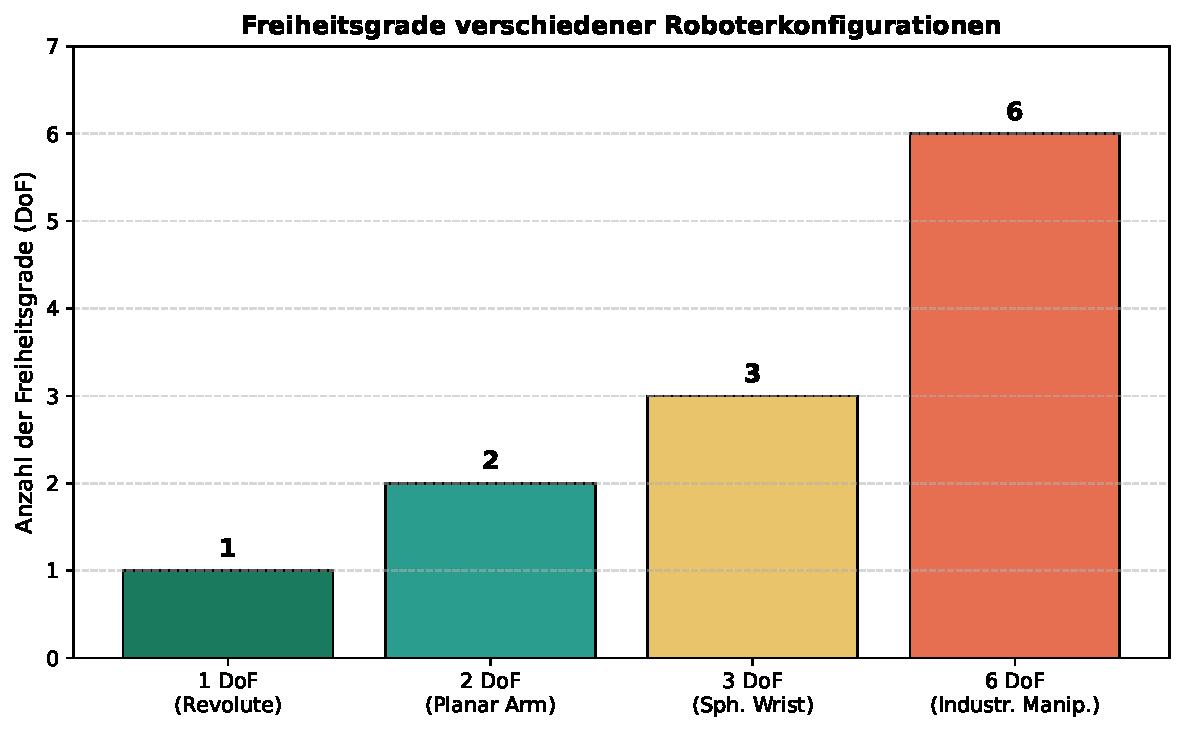
\includegraphics[width=0.75\textwidth]{plot1_dof_comparison.pdf}
	\caption{Vergleich der Freiheitsgrade verschiedener Roboterkonfigurationen. Die vier Konfigurationen
	zeigen den stufenweisen Anstieg von 1 DoF (einfaches Drehgelenk) bis 6 DoF (Industriemanipulator).
	Der sprunghafte Anstieg von 3 auf 6 DoF reflektiert die kombinierte Anforderung an
	Position und Orientierung im dreidimensionalen Raum.}
	\label{fig:dof_compare}
\end{figure}

\subsection{Arbeitsraum als Funktion der Freiheitsgrade}

Abbildung~\ref{fig:workspace} veranschaulicht die qualitative Zunahme des erreichbaren Arbeitsraumvolumens mit steigender Anzahl an Freiheitsgraden. Während ein 1-DoF-System lediglich auf einer Kreislinie operiert, deckt ein 6-DoF-System (normiert auf 1) den gesamten erreichbaren Raum ab.

\begin{figure}[h]
	\centering
	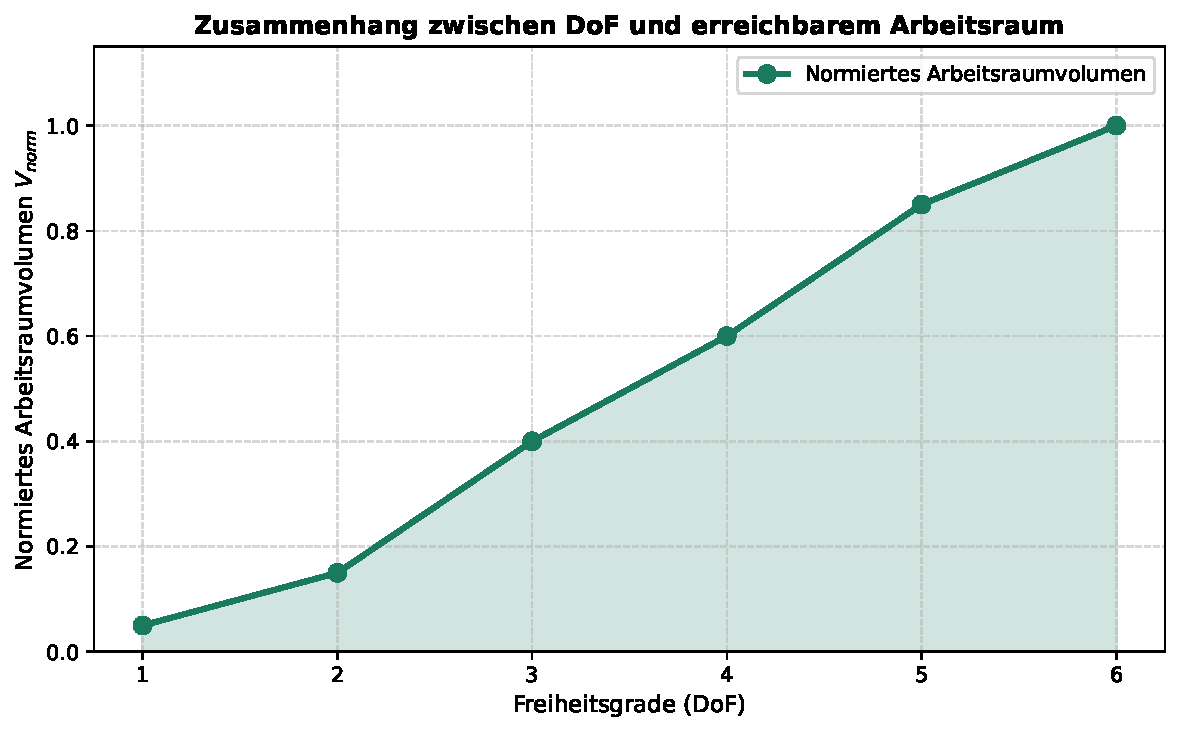
\includegraphics[width=0.75\textwidth]{plot2_workspace_vs_dof.pdf}
	\caption{Normiertes Arbeitsraumvolumen als Funktion der Freiheitsgrade. Die Kurve verdeutlicht, dass
	schon ab 3 DoF ein signifikanter Anteil des dreidimensionalen Arbeitsraums abgedeckt wird. Der
	steile Anstieg zwischen 1 und 3 DoF spiegelt den Übergang von planarer zu räumlicher Erreichbarkeit wider.}
	\label{fig:workspace}
\end{figure}

\subsection{Rotationsmatrizen}

Abbildung~\ref{fig:rotmats} zeigt die nichtlinearen Verläufe der Matrixeinträge der drei elementaren Rotationsmatrizen $R_x$, $R_y$ und $R_z$ als Funktion des Winkels $\theta \in [0, 2\pi]$. Die periodischen Kosinus- und Sinusfunktionen bestimmen die wesentlichen kinematischen Eigenschaften der Gelenke.

\begin{figure}[h]
	\centering
	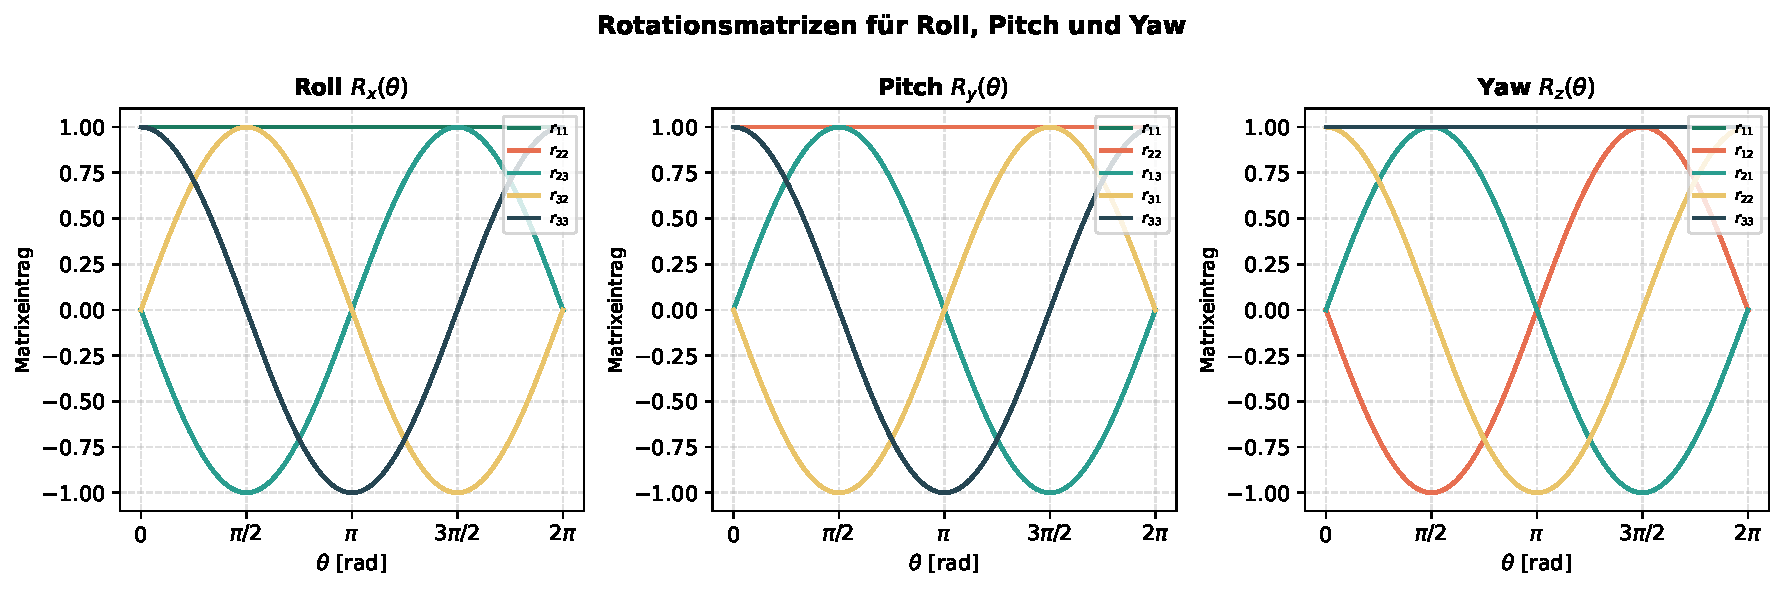
\includegraphics[width=\textwidth]{plot3_rotation_matrices.pdf}
	\caption{Matrixeinträge der elementaren Rotationsmatrizen $R_x(\phi)$ (Roll), $R_y(\theta)$ (Pitch)
	und $R_z(\psi)$ (Yaw) für $\theta \in [0, 2\pi]$. Die Einheitseinträge (konstant 1) auf der
	Hauptdiagonale markieren die Rotationsachse; alle anderen Einträge variieren harmonisch.}
	\label{fig:rotmats}
\end{figure}

\subsection{Kombinatorische Komplexität der Konfigurationen}

Abbildung~\ref{fig:complexity} vergleicht die kombinatorische Komplexität bei naiver Permutationssuche ($n!$) gegenüber dem Ansatz mit zyklischen Rotationen ($n$). Dies ist relevant für die Analyse der Gelenkzustandsräume in der Bahnplanung.

\begin{figure}[h]
	\centering
	
\includegraphics[width=0.75\textwidth]{plot4_complexity.pdf}
	\caption{Vergleich der kombinatorischen Komplexität: naive Permutationssuche ($n!$, rote Quadrate)
	gegenüber zyklischen Rotationen ($n$, grüne Kreise) auf logarithmischer Skala. Für $n=8$ übersteigt
	die Permutationsanzahl ($8! = 40320$) die Rotationsanzahl ($8$) um den Faktor $5040$, was den
	Vorteil strukturierter Suchstrategien quantifiziert.}
	\label{fig:complexity}
\end{figure}

\subsection{Denavit-Hartenberg-Parameter}

Abbildung~\ref{fig:dh} stellt die vier DH-Parameter aller sechs Gelenke eines exemplarischen 6-DoF-Industrieroboters (PUMA-ähnliche Kinematik) als Heatmap dar.

\begin{figure}[h]
	\centering
	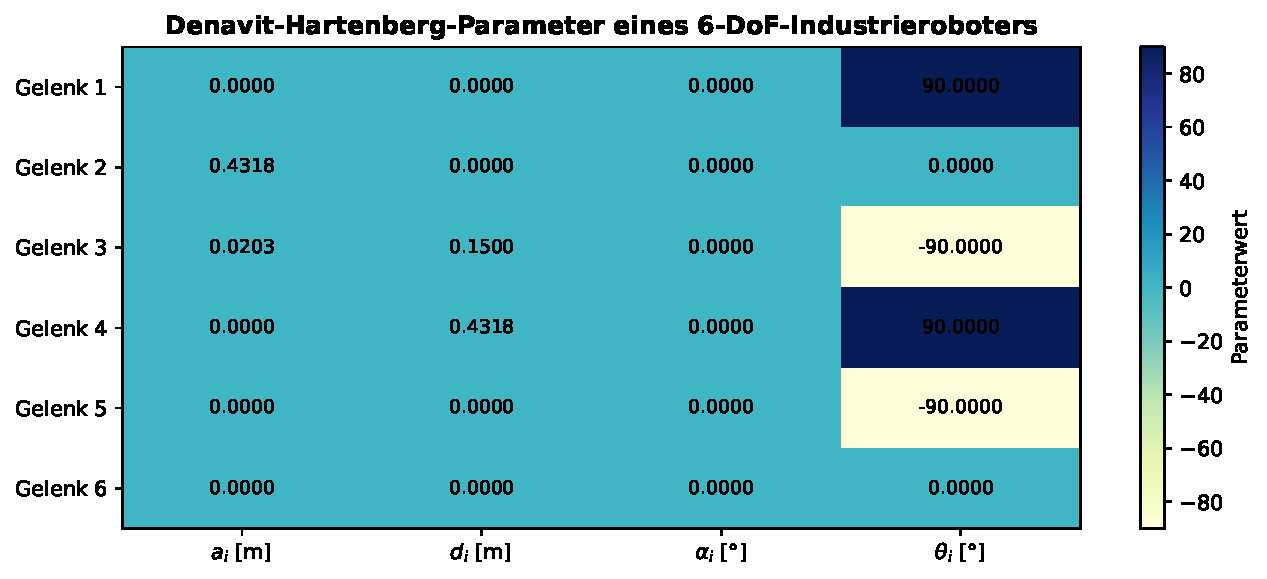
\includegraphics[width=\textwidth]{plot5_dh_params.pdf}
	\caption{Denavit-Hartenberg-Parameter eines 6-DoF-Industrieroboters. Die vier Spalten zeigen
	Gliedlänge $a_i$, Gelenkversatz $d_i$, Gliedverdrehung $\alpha_i$ und Gelenkwinkel $\theta_i$
	für die sechs Gelenke. Gelenke mit $\alpha_i \neq 0$ sind für Richtungsänderungen der
	kinematischen Kette verantwortlich.}
	\label{fig:dh}
\end{figure}

\subsection{Konditionszahl der Jacobi-Matrix}

Abbildung~\ref{fig:jacobian} zeigt die Konditionszahl $\kappa(J) = \|J\|\cdot\|J^+\|$ der Jacobi-Matrix eines 2-DoF-Planar-Arms als Funktion des zweiten Gelenkwinkels $\theta_2$. Hohe Konditionszahlen indizieren Nähe zu kinematischen Singularitäten.

\begin{figure}[h]
	\centering
	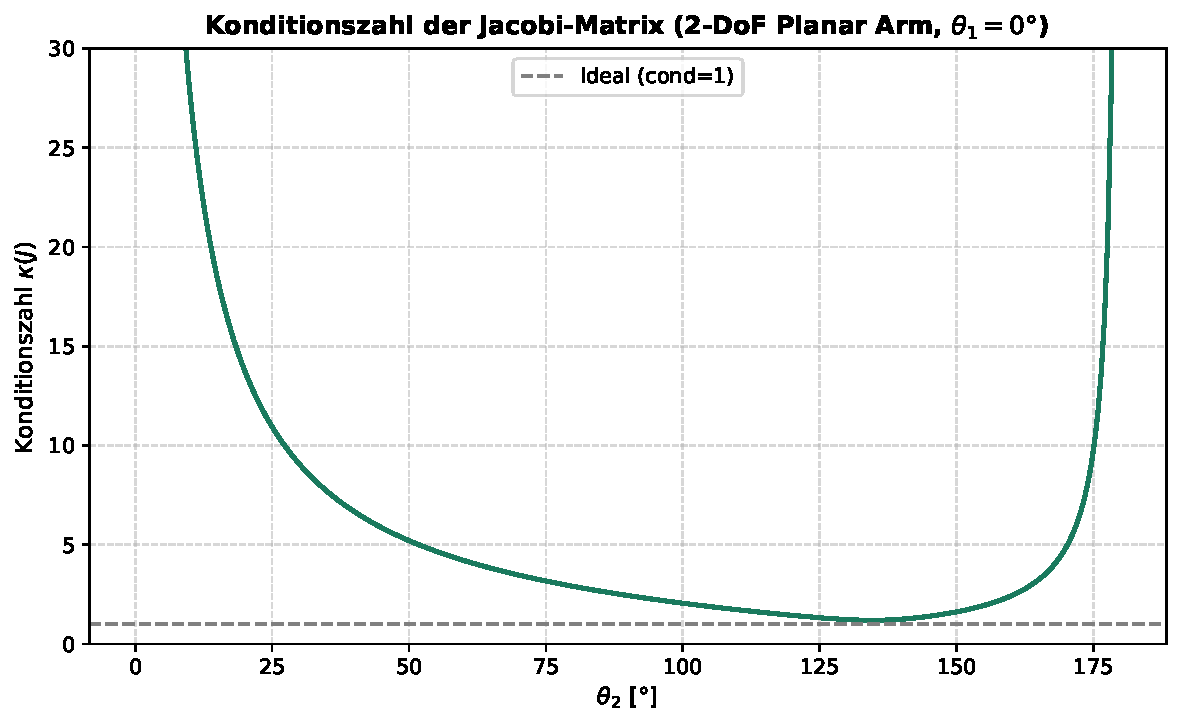
\includegraphics[width=0.75\textwidth]{plot6_jacobian_condition.pdf}
	\caption{Konditionszahl der Jacobi-Matrix des 2-DoF-Planar-Arms ($\ell_1 = 1{,}0\,\text{m}$,
	$\ell_2 = 0{,}8\,\text{m}$, $\theta_1 = 0{}^\circ$) als Funktion von $\theta_2 \in (0{}^\circ, 180{}^\circ)$.
	Die Konditionszahl divergiert für $\theta_2 \to 0{}^\circ$ (vollständig gestreckter Arm), was die
	Singularität nach Satz~\ref{satz:singular} bestätigt. Für $\theta_2 \approx 90{}^\circ$ wird das
	Minimum erreicht, was einer gut konditionierten Konfiguration entspricht.}
	\label{fig:jacobian}
\end{figure}

% ============================================================
\section{Zusammenfassung}
% ============================================================

Diese Arbeit hat die Freiheitsgrade in der Robotik systematisch auf Basis formaler kinematischer Grundlagen entwickelt. Die Grübler-Formel (Satz~\ref{satz:gruebler}) liefert das allgemeine Werkzeug zur DoF-Berechnung beliebiger Mechanismen. Die Vorwärtskinematik planarer und räumlicher Manipulatoren wurde explizit hergeleitet, und ihre Invertierbarkeit sowie Singularitäten wurden formal analysiert. Die mathematische Struktur $SE(3) = SO(3) \ltimes \mathbb{R}^3$ erklärt, warum genau 6 Freiheitsgrade für vollständige räumliche Aufgaben erforderlich sind (Satz~\ref{satz:se3dim}).

\subsection{Ergebnisse im Überblick}

\begin{itemize}
	\item \textbf{1 DoF (Revolutes Gelenk):} Kreisförmiger Arbeitsraum, homogene Transformation $T(\theta) \in SE(3)$.
	\item \textbf{2 DoF (Planarer Arm):} Annulärer Arbeitsraum mit innerer Grenze $|\ell_1-\ell_2|$ und äußerer Grenze $\ell_1+\ell_2$; zwei inverse Kinematik-Lösungen (Ellbogen oben/unten).
	\item \textbf{3 DoF (Sphärisches Handgelenk):} Volle Orientierungskontrolle über $SO(3)$ mit $\dim(SO(3)) = 3$.
	\item \textbf{6 DoF (Industriemanipulator):} Vollständige Positions- und Orientierungskontrolle über $SE(3)$ mit $\dim(SE(3)) = 6$; redundante Roboter ($n > 6$) benötigen Pseudoinverse-Methoden.
\end{itemize}

% ============================================================
\section{Ausblick}
\label{sec:ausblick}
% ============================================================

Die in dieser Arbeit entwickelten Grundlagen eröffnen zahlreiche weiterführende Forschungsrichtungen. Die folgenden Abschnitte skizzieren die wichtigsten offenen Fragen und vielversprechendsten Erweiterungen.

\subsection{Redundante Roboter und Nullraumsteuerung}

Robotersysteme mit $n > 6$ Freiheitsgraden besitzen einen $(n-6)$-dimensionalen \emph{Nullraum} der Jacobi-Matrix, der ohne Beeinflussung der Endeffektor-Pose für Zusatzaufgaben genutzt werden kann. Zu den offenen Fragestellungen gehören die optimale Aufteilung der Gelenkbewegung zwischen Primär- und Sekundäraufgabe sowie Verfahren zur Vermeidung von Gelenklimits, Kollisionen und Singularitäten durch gezielte Nullraumbewegungen \cite{liegeois1977automatic}. Maschinenlernbasierte Ansätze, insbesondere \emph{Reinforcement Learning} \cite{sutton2018reinforcement}, zeigen Potenzial, optimale Nullraumstrategien für spezifische Aufgabenklassen automatisch zu erlernen. Darüber hinaus sind Echtzeitfähige Algorithmen für die Nullraumoptimierung unter harten Zeitbedingungen ein aktives Forschungsfeld \cite{siciliano2009robotics}.

\subsection{Dynamische Modellierung und Echtzeit-Regelung}

Die rein kinematische Betrachtung dieser Arbeit abstrahiert von Massenträgheit, Gelenkreibung und externen Kräften. Die Euler-Lagrange-Formulierung der Roboterdynamik
\[
	M(\mathbf{q})\ddot{\mathbf{q}} + C(\mathbf{q},\dot{\mathbf{q}})\dot{\mathbf{q}} + \mathbf{g}(\mathbf{q}) = \boldsymbol{\tau}
\]
mit Massenmatrix $M$, Coriolis-Matrix $C$, Gravitationsvektor $\mathbf{g}$ und Gelenkdrehmomentvektor $\boldsymbol{\tau}$ bildet die Grundlage für präzise Kraftregelung \cite{spong2020robot}. Moderne modellprädiktive Regelung (MPC) für Robotersysteme erlaubt die simultane Behandlung von kinematischen und dynamischen Beschränkungen und wird künftig durch neuronale Netze zur Modellvorhersage erweitert werden \cite{rawlings2017model}. Insbesondere für hochdynamische Anwendungen wie Sprungbewegungen und schnelle Montageaufgaben bleiben Echtzeit-Lösbarkeit und numerische Stabilität zentrale Herausforderungen.

\subsection{Topologische Aspekte des Konfigurationsraums}

Der Konfigurationsraum eines $n$-Gelenk-Revolute-Roboters ist der $n$-Torus $\mathbb{T}^n = (S^1)^n$. Die globale Topologie dieses Raums beeinflusst wesentlich die Bahnplanung: Wege auf $\mathbb{T}^n$ können sich nicht-trivial umwickeln, und schnelle Verbindungspfade zwischen Konfigurationen setzen topologisches Verständnis voraus. Werkzeuge aus der \emph{algebraischen Topologie} wie Homotopiegruppen und Morse-Theorie finden zunehmend Eingang in die Robotik-Bahnplanung \cite{lavalle2006planning}. Ein offenes Problem ist die effiziente Berechnung optimaler Pfade in homotopischen Äquivalenzklassen für hochdimensionale Konfigurationsräume.

\subsection{Weiche Roboter und kontinuierliche Kinematik}

Traditionelle Roboter bestehen aus starren Gliedern mit diskreten Gelenken. \emph{Soft Robotics} untersucht Systeme aus kontinuierlich deformierbaren Materialien, bei denen der Konfigurationsraum unendlichdimensional ist und durch partielle Differentialgleichungen (z.B. Euler-Bernoulli-Balkentheorie) beschrieben wird \cite{rus2015design}. Die Übertragung des DoF-Konzepts auf solche Systeme ist konzeptionell herausfordernd und Gegenstand aktueller Grundlagenforschung. Erste Ansätze modellieren deformierbare Strukturen durch modale Reduktion auf endlichdimensionale Freiheitsgradräume, was eine Brücke zur klassischen Roboterkinematik bildet.

\subsection{Parallele Kinematiken und Stewart-Gough-Plattformen}

Im Gegensatz zu seriellen Kinematiken verbinden \emph{parallele Roboter} Basis und Endeffektor durch mehrere kinematische Ketten gleichzeitig. Die Berechnung der Freiheitsgrade paralleler Mechanismen erfordert erweiterte Varianten der Grübler-Formel und ist im Allgemeinen schwieriger \cite{merlet2006parallel}. Parallele Roboter wie die Stewart-Gough-Plattform erzielen trotz 6 Freiheitsgraden eine deutlich höhere Steifigkeit und Präzision als serielle Manipulatoren, jedoch auf Kosten eines kleineren Arbeitsraums. Die Analyse ihrer Singularitätsmengen und die Entwicklung singularitätsfreier Arbeitsräume sind aktive Forschungsthemen.

\subsection{Sensorbasierte und adaptive Kinematik}

Zukünftige Robotersysteme werden zunehmend sensorbasiert arbeiten und ihre kinematischen Modelle \emph{online} an wechselnde Bedingungen anpassen. Taktile Sensoren, Kraftmomentmessung und visuelle Servoregelung ermöglichen reaktive Kinematiksteuerung \cite{chaumette2006visual}. Adaptive Jacobi-Schätzer, die ohne explizites Modellwissen arbeiten, könnten die Robustheit gegenüber Kalibrierungsfehlern und Verschleiß erhöhen. Maschinelles Lernen, insbesondere \emph{Gaussian Process Regression} zur Modellierung kinematischer Unsicherheiten, gewinnt hier an Bedeutung.

\subsection{Quantenkinematik und neuartige Freiheitsgrade}

Ein spekulativer, aber wissenschaftlich interessanter Ausblick betrifft die Anwendung quantenmechanischer Konzepte auf die Roboterkinematik. Quantenalgorithmen könnten die inverse Kinematik hochdimensionaler redundanter Roboter durch Superpositionsprinzip und Quantenparallelismus exponentiell beschleunigen \cite{biamonte2017quantum}. Zudem eröffnen neue Materialien (Formgedächtnislegierungen, elektroaktive Polymere, pneumatische Aktoren) neuartige kinematische Primitivtypen jenseits klassischer Revolute- und Prisma-Gelenke, die neue Freiheitsgradkonzepte erfordern.

\subsection{Implementierungsaspekte}

Die in dieser Arbeit beschriebenen Algorithmen sind unter \url{https://github.com/hjstephan86/science} als Teil des wissenschaftlichen Portfolios frei verfügbar. Zukünftige Implementierungsarbeiten werden sich auf GPU-parallele Vorwärtskinematik-Berechnungen, Hardware-in-the-Loop-Simulation mit ESP32/MicroPython-basierten Gelenkreglern sowie die Integration in ROS\,2 (Robot Operating System) für echtzeitfähige Robotersteuerung konzentrieren \cite{quigley2009ros}.

% ============================================================
\begin{thebibliography}{99}

\bibitem{denavit1955kinematic}
J. Denavit und R.\,S. Hartenberg.
\newblock A kinematic notation for lower-pair mechanisms based on matrices.
\newblock \emph{ASME Journal of Applied Mechanics}, 22(2):215--221, 1955.

\bibitem{craig2005introduction}
J.\,J. Craig.
\newblock \emph{Introduction to Robotics: Mechanics and Control}.
\newblock 3.\,Auflage. Pearson Prentice Hall, Upper Saddle River, NJ, 2005.

\bibitem{siciliano2009robotics}
B. Siciliano, L. Sciavicco, L. Villani, und G. Oriolo.
\newblock \emph{Robotics: Modelling, Planning and Control}.
\newblock Springer, London, 2009.

\bibitem{spong2020robot}
M.\,W. Spong, S. Hutchinson, und M. Vidyasagar.
\newblock \emph{Robot Modeling and Control}.
\newblock 2.\,Auflage. Wiley, Hoboken, NJ, 2020.

\bibitem{murray1994mathematical}
R.\,M. Murray, Z. Li, und S.\,S. Sastry.
\newblock \emph{A Mathematical Introduction to Robotic Manipulation}.
\newblock CRC Press, Boca Raton, FL, 1994.

\bibitem{lavalle2006planning}
S.\,M. LaValle.
\newblock \emph{Planning Algorithms}.
\newblock Cambridge University Press, Cambridge, UK, 2006.

\bibitem{sutton2018reinforcement}
R.\,S. Sutton und A.\,G. Barto.
\newblock \emph{Reinforcement Learning: An Introduction}.
\newblock 2.\,Auflage. MIT Press, Cambridge, MA, 2018.

\bibitem{liegeois1977automatic}
A. Liegeois.
\newblock Automatic supervisory control of the configuration and behavior of
  multibody mechanisms.
\newblock \emph{IEEE Transactions on Systems, Man, and Cybernetics},
  7(12):868--871, 1977.

\bibitem{merlet2006parallel}
J.-P. Merlet.
\newblock \emph{Parallel Robots}.
\newblock 2.\,Auflage. Springer, Dordrecht, 2006.

\bibitem{rawlings2017model}
J.\,B. Rawlings, D.\,Q. Mayne, und M. Diehl.
\newblock \emph{Model Predictive Control: Theory, Computation, and Design}.
\newblock 2.\,Auflage. Nob Hill Publishing, Santa Barbara, CA, 2017.

\bibitem{rus2015design}
D. Rus und M.\,T. Tolley.
\newblock Design, fabrication and control of soft robots.
\newblock \emph{Nature}, 521(7553):467--475, 2015.

\bibitem{chaumette2006visual}
F. Chaumette und S. Hutchinson.
\newblock Visual servo control, part I: Basic approaches.
\newblock \emph{IEEE Robotics and Automation Magazine}, 13(4):82--90, 2006.

\bibitem{biamonte2017quantum}
J. Biamonte, P. Wittek, N. Pancotti, P. Rebentrost, N. Wiebe, und S. Lloyd.
\newblock Quantum machine learning.
\newblock \emph{Nature}, 549(7671):195--202, 2017.

\bibitem{quigley2009ros}
M. Quigley, K. Conley, B. Gerkey, J. Faust, T. Foote, J. Leibs, R. Wheeler,
  und A.\,Y. Ng.
\newblock ROS: an open-source robot operating system.
\newblock In \emph{ICRA Workshop on Open Source Software}, Band~3, Seite~5,
  2009.

\bibitem{grubler1917theorie}
M. Gr{\"u}bler.
\newblock \emph{Getriebelehre: Eine Theorie des Zwanglaufes und der ebenen
  Mechanismen}.
\newblock Springer, Berlin, 1917.

\end{thebibliography}

\end{document}
